

\section{Production LMs for Mobile Keyboard} \label{sec:gboard}


%%%%%%%%%%%%%%%%%%%%%%%%%%
\begin{table*}[thb]
    \centering
    \small
    \begin{tabular}{c|c|c|c|c|c|c|c}
         \hline
         \multirow{2}{*}{LM} & \multirow{2}{*}{Rnds} & \multicolumn{3}{c|}{Utility} & \multicolumn{3}{c}{Privacy} \\
         \cline{3-8}
           & & NWP(\%) & WMR(-\%) & WPM(+\%)   & Mech-$\sigma$/MinS/MaxP & zCDP & DP-$ \epsilon$ \\
         \hline
         \multirow{2}{*}{es-ES} & \multirow{2}{*}{1280} & 14.07 $\pm$ 0.06 &  - & - 
            & \bandmf-1.411 / 296 / 4  & 0.29 & 4.82  \\
            & &  13.98 $\pm$ 0.11 & 0.38 & 0.13 & \blt-7.379 / 300 / 4 & 0.16 & 3.46 \\
         \hline
          \multirow{2}{*}{id-ID} & \multirow{2}{*}{2350} & 5.80 $\pm$ 0.10 &  -  & - 
            & \treeagg-7 / 437 / 5  & 0.94 & 9.29  \\
            & & 5.87 $\pm$ 0.04  & 0.09 & 0.07 & \blt-7.379 / 447 / 5 & 0.20 & 3.93 \\
         \hline
         \multirow{3}{*}{pt-BR} & \multirow{3}{*}{2000} & 13.77 $\pm$ 0.36 &  - & - 
            & \bandmf-4.523 / 2001 / 1  & 2.45e-2 & 1.32  \\
            & & 13.86 $\pm$ 0.25 & {\color{gray} -0.04} & 0.04 & \blt-8.681 / 2001 / 1 & 2.23e-2 & 1.25 \\
            & & 13.96 $\pm$ 0.18 & {\color{gray}-0.13} & 0.18 & \blt-16.1 / 1181 / 2 & 1.40e-2 & 0.98 \\
         \hline
         \multirow{3}{*}{pt-PT}  & 430 & 13.58 $\pm$ 0.06 & - & -  
         & \treeagg-7 / 91 / 4 & 1.33 & 11.27 \\
         & 430 & 13.76 $\pm$ 0.11 & 0.38 & {\color{gray} -0.24} & \blt-3.12 / 92 / 4 & 1.11 & 10.19\\
         & 320 & 13.66 $\pm$ 0.04 & 0.07 & {\color{gray} -0.12} & \blt-5.5 / 49 / 6 & 0.75 & 8.19\\
         \hline
    \end{tabular}
    \caption{\small Privacy and utility of production LMs. Utility are measured by NWP accuracy averaged between $r\pm50$ rounds for round $r$ ($r\pm10$ for pt-PT), and the relative WMR decrease and WPM increase in A/B test; privacy shows the key parameters and corresponding DP guarantees, and smaller DP guarantees represent stronger protection; DP-$\epsilon$ is accounted for small $\delta=10^{-10}$; estimated population sizes are es-ES (4.21M), id-ID (8.9M), pt-BR (16.6M), and pt-PT (0.83M). We run additional experiments on pt-BR and pt-PT with larger noise multipliers linearly scales with larger report goal for the \blt mechanism. }
    \vspace{-0.4cm}
    \label{tab:gboard}
\end{table*}

%%%%%%%%%%%%%%%%%%%%%%%%

\paragraph{Production Setting} Our BLT-DP-FTRL algorithm is flexible in min-sep (shown in \cref{sec:rmse_exp}), achieves competitive privacy-utility performance for relatively large signal-to-noise ratio (shown in \cref{sec:sonwp}), and saves computation and memory cost (shown in \cref{tab:mechanism_summary}), which motivates the usage in production FL systems. 
\ifthenelse{\boolean{acl}}{ We follow~\citep{xu2023federated} for the production setting, and provide additional details including the configuration for baselines in \cref{app:prod_config}.
}{
Following \citet{hard2018gboard,xu2023federated}, we train one-layer LSTM LMs of $\sim6.4M$ parameters for mobile keyboard applications. These LMs are deployed on device to predict words during decoding time to facilitate user typing. 
We use next word prediction (NWP) accuracy on a hold-out set of devices to track the training progress, and also conduct A/B test in production, where following two metrics are reported:
\begin{enumerate*}[label=\color{purple}(\arabic*)]
    \item Word Modified Ratio (WMR), the ratio of words being modified during typing or after committed; improvement is shown by reduction;
    \item Word Per Minute (WPM): the number of committed words per minute.
\end{enumerate*}
LMs are trained for different language-locale combination in different populations. We study Spanish in Spain (es-ES), Indonesian in Indonesia (id-ID), Portuguese in Brazil (pt-BR) and Portuguese in Portugal (pt-PT). LMs are pre-trained on public multilingual C4 dataset~\citep{xue2020mt5} before private training with FL and DP. 

\paragraph{Algorithm Setting} We compare our BLT-DP-FTRL algorithm with \treeagg~\citep{kairouz21practical,xu2023federated} and \bandmf~\citep{choquette2023amplified} discussed in \cref{sec:background}. As far as we know, these two are the only DP algorithms actively used to train LMs in a production FL system. We follow the system and parameter configurations in~\citep{xu2023federated,choquette2023amplified,gboard_dp_blogpost} for baselines, and compare to \treeagg for pt-PT and id-ID, and \bandmf for es-ES and pt-BR. However, we highlight it is challenging to exactly reproduce the settings, especially for the min-sep parameter. The \bandmf algorithm are optimized for total round $n=2000$, band $\hat b = 400$ for es-ES, and $\hat b = 1000$ for pt-BR. We optimize \blt for total round $n=4000$\footnote{As the target round is usually less than 2000, $n=4000$ for \blt is less favorable compared to $n=2000$ used for \bandmf. \blt is robust to the target round $n$, and achieves stronger results with an inferior $n$.}, estimated min-sep $b=100$ for pt-PT, $b=400$ for es-ES and id-ID, and $b=1000$ for pt-BR. We use \ourblt for multi-participation and estimate the max-par based on $n/b$. For these $n,b$ settings, only $d=4$ buffers can achieve near-optimal loss in optimization, and \ourblt matrices are parameterized by only 8 numbers (these parameters are provided in \cref{app:blt_params}). Though different configures are used for populations with different sizes, the BLT parameters $(\theta, \outp) \in \R^8$ optimized for $b=400$ can achieve competitive results for a wide range of min-seps, which can be a reasonable default for BLT-DP-FTRL. As discussed in \cref{tab:mechanism_summary}, \blt is more memory-efficient than both \treeagg and \bandmf. In the simulation results \cref{tab:sonwp}, \blt is also better than \treeagg for privacy-utility trade-off, and comparable with \bandmf. The results in production further show that the flexibility of \blt makes it easier to use in practice, and achieve better results than both \treeagg and \bandmf.
}
%%%%%%%%%%%%%%%%%%%%%%%%%%%%%%%%%%%%%%%%
\begin{figure}[thb]
\centering
\begin{subfigure}[b]{0.45\linewidth}
\centering
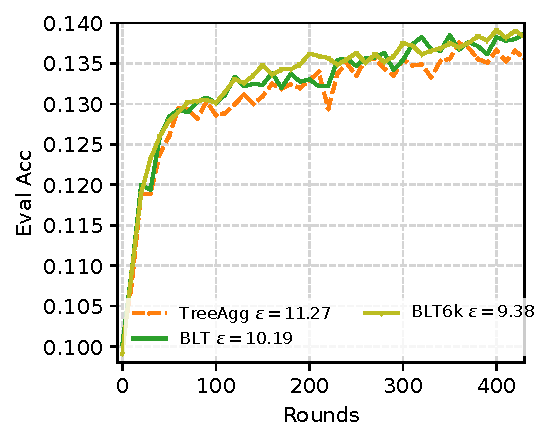
\includegraphics[width=\textwidth]{images/ptpt_acc.pdf}
\caption{\small NWP \ifthenelse{\boolean{acl}}{}{evaluation} accuracy}
\label{fig:example_acc}
\end{subfigure}
%
\begin{subfigure}[b]{0.44\linewidth}
\centering
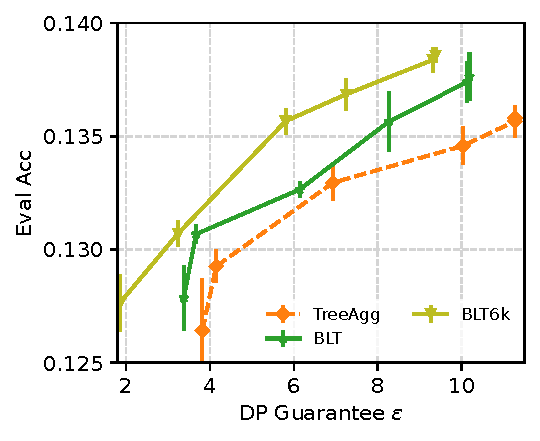
\includegraphics[width=\textwidth]{images/ptpt_priv.pdf}
\caption{\small Privacy-utility trade-off}
\label{fig:example_priv}
\end{subfigure}
%
\ifthenelse{\boolean{acl}}{
\caption{\small NWP evaluation accuracy and the dervied privacy-utility trade-off curves for training the Portuguese LM in Portugal (pt-PT) with DP-FTRL in a FL system. Additional curves for es-ES, id-ID, and pt-BR are provided in \cref{fig:acc_curve,fig:acc_curve2,fig:priv_curve}. \blts achieve better privacy-utility trade-off.}
}{
\caption{\small NWP evaluation accuracy and privacy-utility trade-off curves for training the production Portuguese LM in Portugal (pt-PT) with DP-FTRL in a FL system. Additional curves for es-ES, id-ID, and pt-BR are provided in \cref{fig:acc_curve,fig:priv_curve}, with NWP accuracy zoomed-in for later stage of training in \cref{fig:acc_curve2}. The privacy-utility trade-off curves are derived from NWP accuracy curves: for each selected round $r$, we compute the mean and standard deviation (shown as vertical bars) for accuracy from the rounds in the range of $r\pm10$, and accounting the DP guarantees. \blts achieve better privacy-utility trade-off.}
}\label{fig:example_curve}
\vspace{-0.4cm}
\end{figure}
%%%%%%%%%%%%%%%%%%%%%%%%%%%%%%%%%%%%%%%%


\ifthenelse{\boolean{acl}}{\textbf}{\paragraph}{Main Results} We summarize the privacy and utility results for es-ES, id-ID, pt-BR, and pt-PT LMs in \cref{tab:gboard}, and show the privacy-utility curves for training pt-PT in \cref{fig:example_curve}. We provide additional curves for other LMs in \cref{fig:acc_curve,fig:acc_curve2,fig:priv_curve} in\cref{app:plots}, and discuss the observations here.
\begin{enumerate*}[label=\color{purple}(\arabic*)]
    \item \emph{Most of the models achieve DP guarantee of $\epsilon<10$ with exception of $\epsilon \sim 10$ for pt-PT due to the challenge of small population; the pt-BR model trained with \blt-16.1 achieves $\epsilon<1$ at round 2000.} DP guarantees of $\epsilon<10$ is commonly used for machine learning, and $\epsilon<1$ are considered strong guarantees~\citep{ponomareva2023dpfy}. To achieve single-digit DP guarantees in practice without sacrificing the utility, the production LMs are trained with large number of clients per round (known as report goal in FL systems). We use typical report goal 6.5K~\citep{xu2023federated} for es-ES, id-ID and pt-BR, and use a smaller report goal 3K for pt-PT with a smaller population. We additionally run BLT-DP-FTRL with larger report goal and linearly scale up the noise multiplier to keep the signal-to-noise ratio for utility: \blt-16.1 with report goal 12K for pt-BR and \blt-5.5 with report goal 6K for pt-PT. The resulting min-seps in pt-BR and pt-PT almost halved when the report goals are increased. We use noise multiplier 7 for \treeagg, which is determined by StackOverflow simulation experiments~\citep{xu2023federated}. \ifthenelse{\boolean{acl}}{}{The noise multiplier of \bandmf is computed so that the RMSE is similar to \treeagg with noise multiplier 7~\citep{choquette2023amplified} and will achieve stronger DP guarantees. As \blt achieves comparable privacy-utility trade-off as \bandmf in the high single-to-noise ratio regime ($\epsilon=8$) in simulation experiment (\cref{tab:sonwp} ), the noise multiplier of \blt is computed so that \blt achieves similar DP guarantee as \bandmf for the desired round.}
    \item \emph{\blt achieves better privacy-utility trade-off compared to \treeagg and \bandmf.} \blt achieves comparable and slightly better NWP accuracy for the models in \cref{tab:gboard} and  \cref{fig:example_curve}, and stronger DP guarantees. The model performance are further verified by A/B test in the production application comparing \blt models to baseline models for WMR and WPM, where we target on improved or neutral utilities. The advantage of \blt in privacy-utility trade-off is clearly demonstrated in \cref{fig:priv_curve}, and \blt is better than not only \treeagg, but also \bandmf across the production LM training. 
    The practical min-sep can be quite different from the estimated min-seps for optimizing \bandmf and \blt matrices, \ifthenelse{\boolean{acl}}{e.g., $\sim$300 compared to 400 for es-ES, and 2000+ compared to 1000 for pt-BR}{$\sim$90 compared to 100 for pt-PT,  $\sim$300 compared to 400 for es-ES, $\sim$440 compared to 400 for id-ID, and 2000+ compared to 1000 for pt-BR}. As \blt is more flexible on min-sep estimation, the challenge of reliably estimating min-sep resulting in \blt achieving even stronger privacy-utility trade-offs than \bandmf in the production LMs training. 
\end{enumerate*}

\ifthenelse{\boolean{acl}}{ 
\textbf{Extrapolation} We extrapolate the results for production setting by assuming linearly increase report goal and noise multiplier, and changing min-sep will not change the utility, and hence we can study the effect on DP without actually training the model. We provide results and detailed discussion in \cref{app:extrap}, which further demonstrate the advantages of BLT-DP-FTRL. 
}{
%%%%%%%%%%%%%%%%%%%%%%%%%%%%%%%%%%%%%%%%
\begin{figure}[thb]
\centering
% 
\begin{subfigure}[b]{0.45\linewidth}
\centering
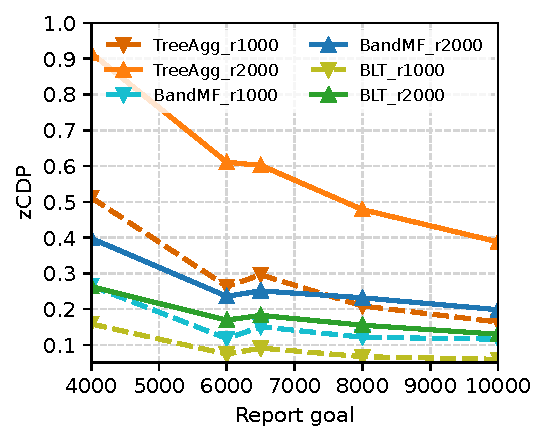
\includegraphics[width=\textwidth]{images/blt_pop3m.pdf}
\caption{\small Population 3M}
\label{fig:pop3m}
\end{subfigure}
%
\begin{subfigure}[b]{0.45\linewidth}
\centering
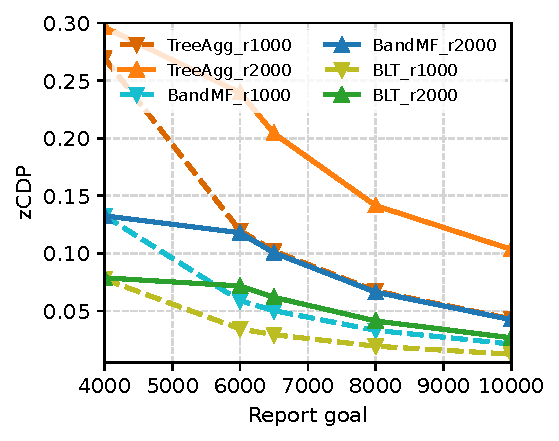
\includegraphics[width=\textwidth]{images/blt_pop10m.pdf}
\caption{\small Population 10M}
\label{fig:pop10m}
\end{subfigure}
%
\begin{subfigure}[b]{0.45\linewidth}
\centering
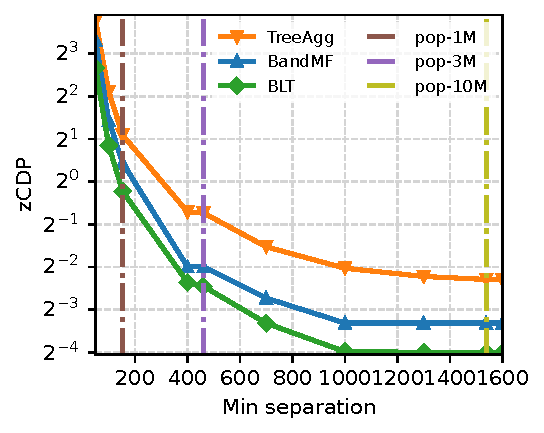
\includegraphics[width=\textwidth]{images/blt_min_sep.pdf}
\caption{\small Report goal 6500, worst-case max-par}
\label{fig:min_sep}
\end{subfigure}
%
\begin{subfigure}[b]{0.45\linewidth}
\centering
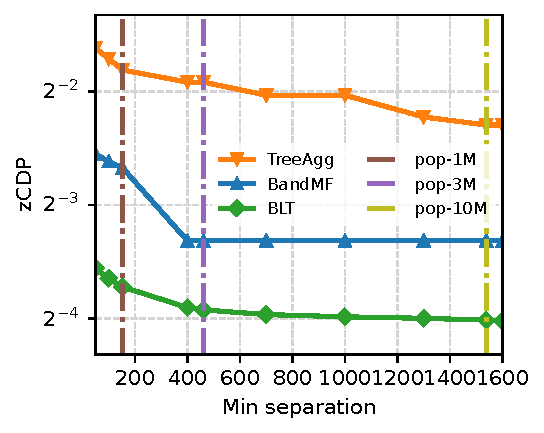
\includegraphics[width=\textwidth]{images/min_sep_max2.pdf}
\caption{\small Report goal 6500, optimistic max-par=2}
\label{fig:min_sep_max2}
\end{subfigure}
%
\caption{\small The effect of population size, number of rounds, report goals, and min-seps on DP-FTRL privacy guarantees. The results are extrapolate from the setting for es-ES and id-ID (\bandmf and \blt matrices are optimized for min-sep=400) based on the hypothesis that linearly scale noise multiplier and report goal, or only change min-sep will not affect the model utility. The For a fixed number of rounds to achieve utility target, increasing report goal and min-sep can achieve stronger guarantees measured by smaller zCDP. The optimal min-sep is capped by population size for a fixed report goal, and \blt provides better guarantees, and smoother transition across different min-seps. 
}\label{fig:extrapolate}
\end{figure}
%%%%%%%%%%%%%%%%%%%%%%%%%%%%%%%%%%%%%%%%

\paragraph{Extrapolation} We extrapolate the results for production setting by using a common hypothesis: linearly increase report goal and noise multiplier will not change the utility of the model as the signal-to-noise ratio is maintained. In addition, we assume only changing min-sep will not change the utility because of the signal-to-noise ratio. The hypothesis has been verified in previous work~\citep{kairouz21practical} and the large report goal experiments for pt-BR and pt-PT in \cref{tab:gboard} and \cref{fig:acc_curve}. Hence we can study the effect on DP without actually training the model, similar to \cref{sec:rmse_exp} for simulation.

We vary the report goal, and the min-sep is optimistically estimated by \emph{min-sep=$\lfloor$population-size/report-goal$\rfloor$}, and \emph{max-par=$\lceil$total-rounds/min-sep$\rceil$} is used unless otherwise specified. We discuss the extrapolation results in \cref{fig:extrapolate}, where utility is the same based on the hypothesis.
\begin{enumerate*}[label=\color{purple}(\arabic*)]
\item \blt achieves better DP guarantees because of its robustness to min-seps and total rounds. 
\item We observe that using larger report goal and optimizing for the largest possible min-sep achieves better results than using smaller report goals and larger corresponding min-sep, similar to observation for \treeagg in \citep{xu2023federated}.
\item \cref{fig:pop10m} shows training more rounds does not necessarily increasing DP guarantees when min-sep is large.
\item The gap of \blt and \bandmf is small when min-sep is accurately estimated. In the regime of relatively high signal-to-noise ratio (large noise multiplier for limited computation resources), \blt is competitive in a wide range of different configurations. Hence \blt is easier to use in production FL systems compared to \bandmf, and also saves memory during training.
\end{enumerate*}

Finally, in \cref{fig:varyn}, we extrapolate the DP guarantee results by varying the number of total rounds $n$ with the noise multiplier for the fixed report goal $6500$, fixed min separation $b=100,400,1000$, and corresponding max participation $k= n / b$. The \treeagg, \blt and \bandmf mechanisms used in production are compared. Instead of using \rmsloss or \maxloss to measure privacy-utility trade-offs in \cref{fig:rmse,fig:rmse_vary_n}, here we fix utility based on empirical utility of the production training and the signal-to-noise-ratio hypothesis, and compare the DP guarantees. As mentioned before, using \bandmf beyond the optimized matrices for $n=2000$ has not been studied before, and hence we only extrapolate \bandmf up to $n=2000$ rounds. \treeagg and \blt can run arbitrary number of rounds, and \blts achieve stronger DP guarantees than \treeagg. In practice, we can use one of the BLTs as a default mechanism across different settings, and perform on-the-fly optimization for given customized setting.  

\begin{figure}[thb]
\centering
\begin{subfigure}[b]{0.325\linewidth}
\centering
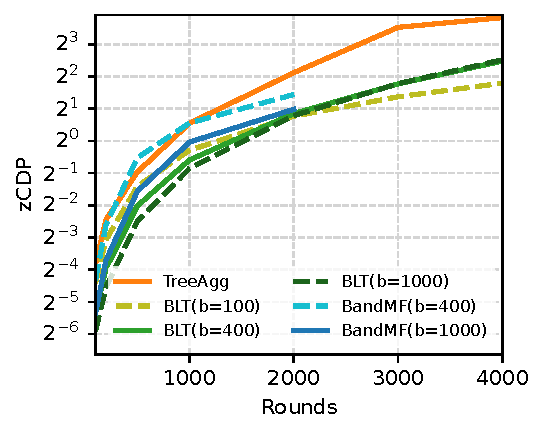
\includegraphics[width=\textwidth]{images/varyn_b100.pdf}
\caption{\small Min-sep b=100}
\label{fig:varyn_b100}
\end{subfigure}
%
\begin{subfigure}[b]{0.33\linewidth}
\centering
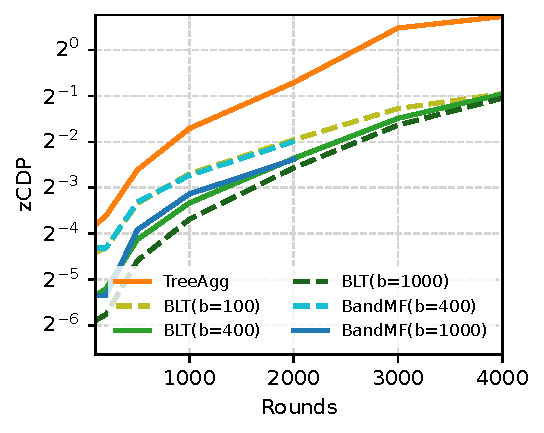
\includegraphics[width=\textwidth]{images/varyn_b400.pdf}
\caption{\small Min-sep b=400}
\label{fig:varyn_b400} 
\end{subfigure}
%
\begin{subfigure}[b]{0.33\linewidth}
\centering
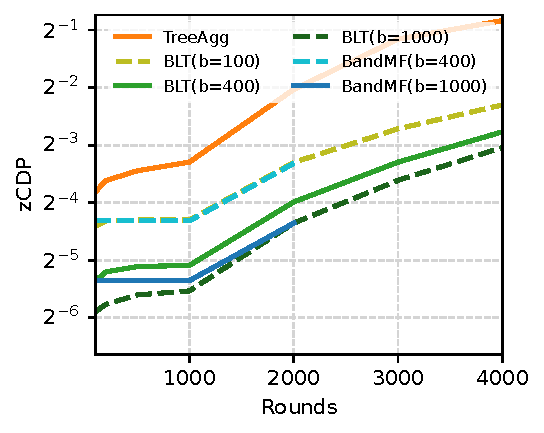
\includegraphics[width=\textwidth]{images/varyn_b1000.pdf}
\caption{\small Min-sep b=1000}
\label{fig:varyn_b1000} 
\end{subfigure}
%
\caption{\small Extrapolate by varying number of rounds $n$ for the \treeagg, \blt and \bandmf mechanisms used in production. Use the noise multiplier for the fixed report goal $6500$; fix min separation $b=100,400,1000$, respectively; worst-case max participation is varied assuming fixed population size, i.e., $k= n / b$. The utility of different mechanisms at a specific round (x-axis value) are assumed to be similar due to the signal-to-noise ratio hypothesis, and we can compare the corresponding zCDP guarantees (y-axis value).}\label{fig:varyn}
\end{figure}

\paragraph{Model launches} We have launched several language models for on-the-fly (OTF) rescoring words in Gboard smart completion and suggestion~\citep{gboard_dp_blogpost,xu2023federated}. The models trained with BLT-DP-FTRL algorithm in this paper achieved better privacy-utility trade-off than the \treeagg-DP-FTRL algorithm~\citep{kairouz21practical} widely used in FL practice~\citep{xu2023federated}, and comparable with MF-DP-FTRL~\citep{choquette2023amplified} that achieves state-of-the-art performance and some $\epsilon<1$ models reported in~\citep{gboard_dp_blogpost}. We report $\rho$-zCDP and $(\epsilon, \delta)$-DP of $\delta=10^{-10}$ following~\citet{xu2023federated,gboard_dp_blogpost}; the details of the DP configuration are provided in \cref{app:privacy-guarantees}. The Portuguese OTF LM in Brazil (pt-BR) is launched with DP $\epsilon=1.234$ (alternatively, zCDP $\rho=0.022$);
pt-PT OTF LM is launched with DP $\epsilon=8.19$ (alternatively, zCDP $\rho=0.749$) compared to DP $\epsilon=9.56$ (alternatively, zCDP $\rho=0.99$) in~\citep{xu2023federated}, and significant improvement in WMR of $-0.91\%$; 
es-ES OTF LM is launched with DP $\epsilon=4$ (alternatively, zCDP $\rho=0.202$) compared to DP $\epsilon=9.01$ (alternatively, zCDP $\rho=0.89$) in~\citep{xu2023federated}; the id-ID OTF LM using new vocabulary constructed from~\citep{gboard_fa_blogpost} is launched with DP $\epsilon=2.74$ (alternatively, zCDP $\rho=0.099$), achieving comparable utility and replacing the previous model without DP. In addition, the discussed default BLT mechanism optimized for $b=400$ and noise multiplier 7.379 is used to train and launch more models: the English LM is launched with DP $\epsilon=4.84$ (alternatively, zCDP $\rho=0.29$); the Spanish LM in Argentina is launched with DP $\epsilon=5.73$ (alternatively, zCDP $\rho=0.392$); the Spanish LM in Mexico is launched with DP $\epsilon=11.58$ (alternatively, zCDP $\rho=1.39$); the Spanish LM in other Latin America countries is launched with  DP $\epsilon=6.84$ (alternatively, zCDP $\rho=0.54$). The new Gboard OTF LMs are trained with FL and DP following the commitment in \citep{gboard_dp_blogpost,zhang2023private}. As of May 2025, all existing FL LMs have been replaced with DP FL models, fully realizing our plan in~\citep{zhang2023private}. 
}

